\documentclass[a4paper, 12pt]{article}
\usepackage{fullpage}

\usepackage{amsmath}
\usepackage{amssymb}
\usepackage{amsfonts}
\usepackage{amsthm}
\usepackage{mathtools}
\usepackage{soul}

\usepackage{color}
\usepackage{listings}

\definecolor{mygreen}{rgb}{0.0, 0.5, 0.0}
\definecolor{emphamber}{rgb}{1.0, 0.75, 0.0}
\definecolor{amber}{rgb}{1.0, 0.49, 0.0}
\definecolor{ballblue}{rgb}{0.13, 0.67, 0.8}
\definecolor{gray}{rgb}{0.5, 0.5, 0.5}

\lstdefinestyle{kamyarStyle}{
    basicstyle=\footnotesize\ttfamily,
    keywordstyle=\color{amber},
    stringstyle=\color{mygreen},
    commentstyle=\color{gray},
    breakatwhitespace=false,
    breaklines=true,
    keepspaces=true,
    showspaces=false,
    showstringspaces=false,
    showtabs=false,
}

\lstset{style=kamyarStyle}
\lstset{escapeinside={(*@}{@*)}}

\usepackage{xepersian}

\settextfont{XB Zar}
\ExplSyntaxOn \cs_set_eq:NN \etex_iffontchar:D \tex_iffontchar:D \ExplSyntaxOff
\setmathdigitfont{Yas}

\theoremstyle{definition}
\newtheorem{solution}{پاسخ}[section]
\newtheorem{solutionsection}{مورد}[solution]
\renewcommand{\thesolution}{\arabic{solution}}

\renewcommand{\baselinestretch}{1.3}

\definecolor{OliveGreen}{rgb}{0.84,1,0.64}

\begin{document}

\textbf{حسابگری زیستی؛}

\textbf{حل مسئله فروشنده دوره‌گرد به کمک نقشه خودسازمان‌دهنده؛}

\textbf{کامیار میرزاوزیری؛ 610396152}

\hrulefill

\section{نقشه خودسازمان‌دهنده}

یک کلاس به اسم
\texttt{SOM}
برای پیاده‌سازی نقشه خودسازمان‌دهنده تعریف می‌کنیم. این کلاس به صورت یک شبکه عصبی تعریف می‌شود که
\texttt{input\_size}
ورودی و
\texttt{output\_size}
خروجی دارد و وزن‌های
$w_{i, j}$
برای
$1 \leq i \leq \texttt{output\_size}$
و
$1 \leq j \leq \texttt{input\_size}$
روی آن تعریف شده‌اند.

\subsection{محاسبه}
خروجی
$i$-ام
این شبکه، بر اساس ورودی‌های
$x_1, \dots x_\texttt{imput\_size}$
و وزن‌های شبکه با تابع زیر محاسبه می‌شود.

\[ y_i = \sqrt{\sum_{j=1}^{\texttt{input\_size}} (x_j - w_{i, j})^2}. \]

که همان فاصله اقلیدسی بین دو بردار
$x$
و
$w_i$
می‌باشد.

از آنجا که فاصله اقلیدسی را در بخش‌های دیگری از کد نیز استفاده می‌کنیم، یک تابع کمکی برای محاسبه آن تعریف می‌کنیم.

\LTR
\begin{lstlisting}[language=Python]
def euclidean_distance(a, b):
    return sum([(a[i] - b[i]) ** 2 for i in range(len(a))]) ** .5
\end{lstlisting}
\RTL

حال می‌توانیم متد
\texttt{compute}
را برای این کلاس تعریف کنیم.

\LTR
\begin{lstlisting}[language=Python]
def compute(self, input):
    return [
        euclidean_distance(input, self.w[i])
        for i in range(self.output_size)
    ]
\end{lstlisting}
\RTL

\subsection{خودسازمان‌دادن}
برای یادگیری در نقشه خودسازمان‌دهنده به این صورت عمل می‌کنیم که بعد از محاسبه خروجی‌ها روی ورودی‌ها، اگر کوچک‌ترین خروجی
$y_m$
باشد، بردارهای وزنی که فاصله اقلیدسی آن‌ها از بردار وزن
$w_m$
(بردار وزن‌های کوچک‌ترین خروجی که کلاستر انتخاب‌شده تعبیر می‌شود)
در یک همسایگی کوچک قرار بگیرد را، کمی به بردار ورودی نزدیک می‌کنیم. این کار از طریق فرمول زیر ممکن می‌شود.

\[ \Delta w_{i,j} = \begin{cases}
        \alpha (x_j - w_{i,j}) & \texttt{ed}(w_m, w_i) \leq \nu \\
        0                      & \text{otherwise}.
    \end{cases}
\]

که در آن
$\texttt{ed}$
همان فاصله اقلیدسی دو بردار است. توجه کنیم که در این فرمول از دو پارامتر
$\alpha$
و
$\nu$
استفاده کردیم. می‌توانیم
$\alpha$
را درجه یادگیری و
$\nu$
را آستانه همسایگی بنامیم که پارامترهایی مختص شبکه می‌باشند.

حال می‌توانیم متد
\texttt{self\_optimize}
را برای این کلاس تعریف کنیم.

\LTR
\begin{lstlisting}[language=Python]
def self_optimize(self, input, m):
    for i in range(self.output_size):
        if euclidean_distance(self.w[m], self.w[i]) <= self.nu:
            for j in range(self.input_size):
                self.w[i][j] += self.alpha * (input[j] - self.w[i][j])
\end{lstlisting}
\RTL

\subsection{مقداردهی اولیه}
نهایتا متد
\texttt{\_\_init\_\_}
را برای راه‌اندازی یک
\texttt{instance}
از این کلاس تعریف می‌کنیم.

\LTR
\begin{lstlisting}[language=Python]
def __init__(self, random_range, input_size, output_size, alpha, nu):
    self.input_size = input_size
    self.output_size = output_size
    self.alpha = alpha
    self.nu = nu
    self.w = [
        [randrange(*random_range[i]) for i in range(input_size)]
        for j in range(output_size)
    ]
\end{lstlisting}
\RTL

که در آن وزن‌ها را در ابتدا به صورت تصادفی در بازه داده شده انتخاب می‌کنیم.

\section{خواندن مسئله و ترسیم آن}

حال که شبکه مورد نظر را پیاده‌سازی کردیم. می‌توانیم مسئله را از فایل ورودی بخوانیم و آن را ترسیم کنیم. برای نمایش شهرها و جاده‌ها، کلاسی به اسم
\texttt{Visualizer}
پیاده‌سازی کردیم که کد کامل آن در فایل سورس
\texttt{main.py}
موجود است. یک صفحه
$3 \times 4$
برای نمایش
$12$
نقشه تعریف می‌کنیم.

\LTR
\begin{lstlisting}[language=Python]
visualizer = Visualizer(3, 4)    
\end{lstlisting}
\RTL

شهر را از روی فایل ورودی می‌خوانیم.

\LTR
\begin{lstlisting}[language=Python]
with open(FILE + '.tsp') as f:
    cities = [{'position': tuple(map(float, l.split()[1:3])), 'cluster': None} for l in f.readlines()]
\end{lstlisting}
\RTL

و نهایتا نقشه خام شهرها را ترسیم می‌کنیم.

\LTR
\begin{lstlisting}[language=Python]
visualizer.add(cities, title='Cities')
\end{lstlisting}
\RTL

\begin{center}
    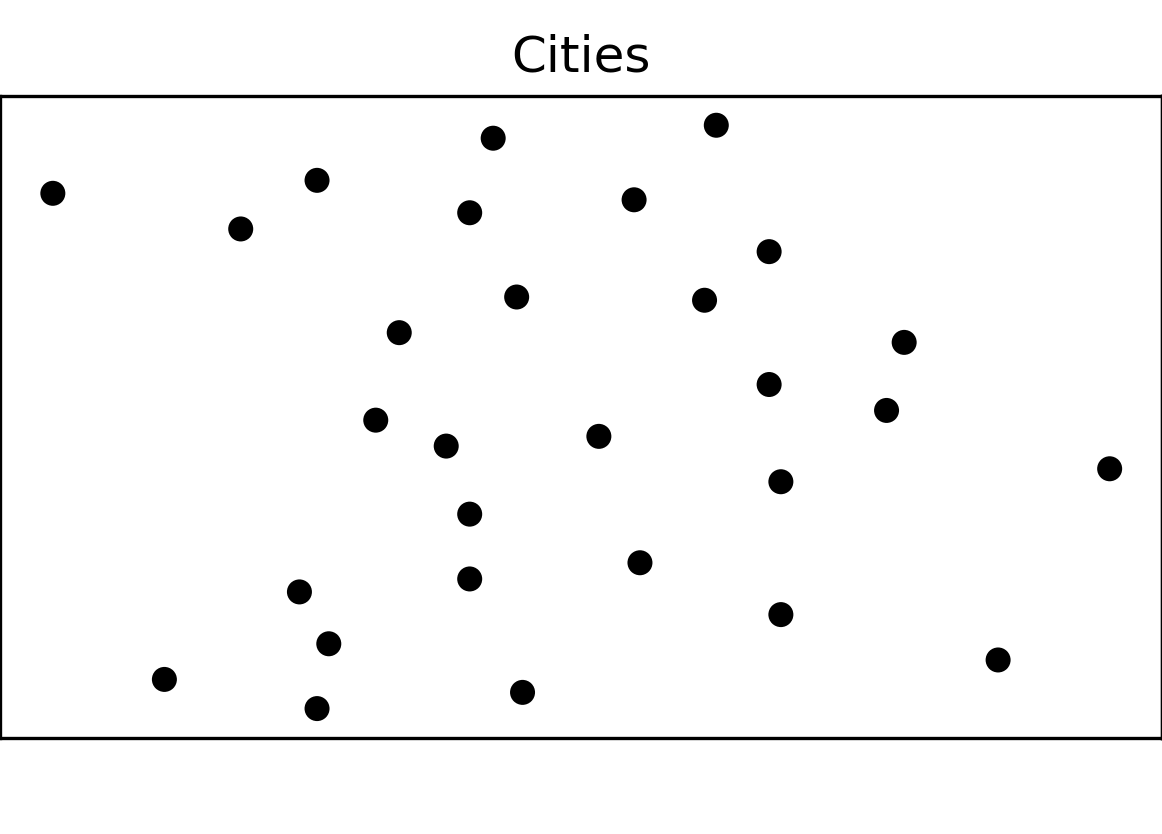
\includegraphics[width=.5\textwidth]{1/0.png}
\end{center}

\section{خوشه‌بندی}

برای خوشه‌بندی به کمک کلاس
\texttt{SOM}
که تعریف کردیم، ابتدا یک
\texttt{instance}
از آن ایجاد می‌کنیم.

\LTR
\begin{lstlisting}[language=Python]
DIMENSION = 2
CLUSTERS_COUNT = 5
ALPHA = .4
NU = 9
RANDOM_RANGE = [
    [min(map(lambda x: x['position'][i], cities)), max(map(lambda x: x['position'][i], cities)) + 1]
    for i in range(DIMENSION)
]
som = SOM(RANDOM_RANGE, DIMENSION, CLUSTERS_COUNT, ALPHA, NU)
\end{lstlisting}
\RTL

ثابت
\texttt{DIMENSION}
که تعداد ورودی‌های شبکه را مشخص می‌کند نشان‌دهنده این است که شهرها در فضای دوبعدی قرار دارند و لذا شامل دو مختصات می‌باشند. باقی پارامتر‌ها و ثابت‌ها به صورت تجربی انتخاب شده‌اند. و بازه‌ای که وزن‌ها را در ابتدا به صورت تصادفی از آن بازه انتخاب می‌کنیم همان بازه‌ای است که مختصات شهرها در آن قرار دارد.

حال در یک حلقه به خوشه‌بندی شهرها می‌پردازیم. هر بار تمام شهرها را خوشه‌بندی می‌کنیم و نقشه خوشه‌بندی‌شده را نصب می‌کنیم. سپس شهرها و خوشه‌های انتخابی را به
\texttt{som}
می‌دهیم تا از آن‌ها یاد بگیرد و خودش را سازمان‌دهی کند. در نهایت درجه یادگیری و آستانه همسایگی را اندکی کم می‌کنیم چرا که در ابتدا وزن‌ها تصادفی انتخاب شده‌اند و یادگیری باید زیاد باشد اما به مرور زمان باید کاهش یابد.

\LTR
\begin{lstlisting}[language=Python]
iteration = 0
while True:
    iteration += 1

    # Cluster each city
    for city in cities:
        som_output = som.compute(city['position'])
        city['cluster'] = som_output.index(min(som_output))

    # Visualize the clustered cities
    visualizer.add(cities, cluster_centers=som.w, title=f'Iteration {iteration}')

    # Learn from each city
    for city in cities:
        som.self_optimize(city['position'], city['cluster'])

    # Lower the degree of learning (alpha)
    # and the threshold of neighborhood (nu)
    som.alpha -= .01
    som.nu -= 1

    # Exit Condition
    if som.alpha <= 0 or som.nu <= 0:
        break
\end{lstlisting}
\RTL

برای مثال در تکرار اول خوشه‌بندی به صورت زیر خواهد بود.

\begin{center}
    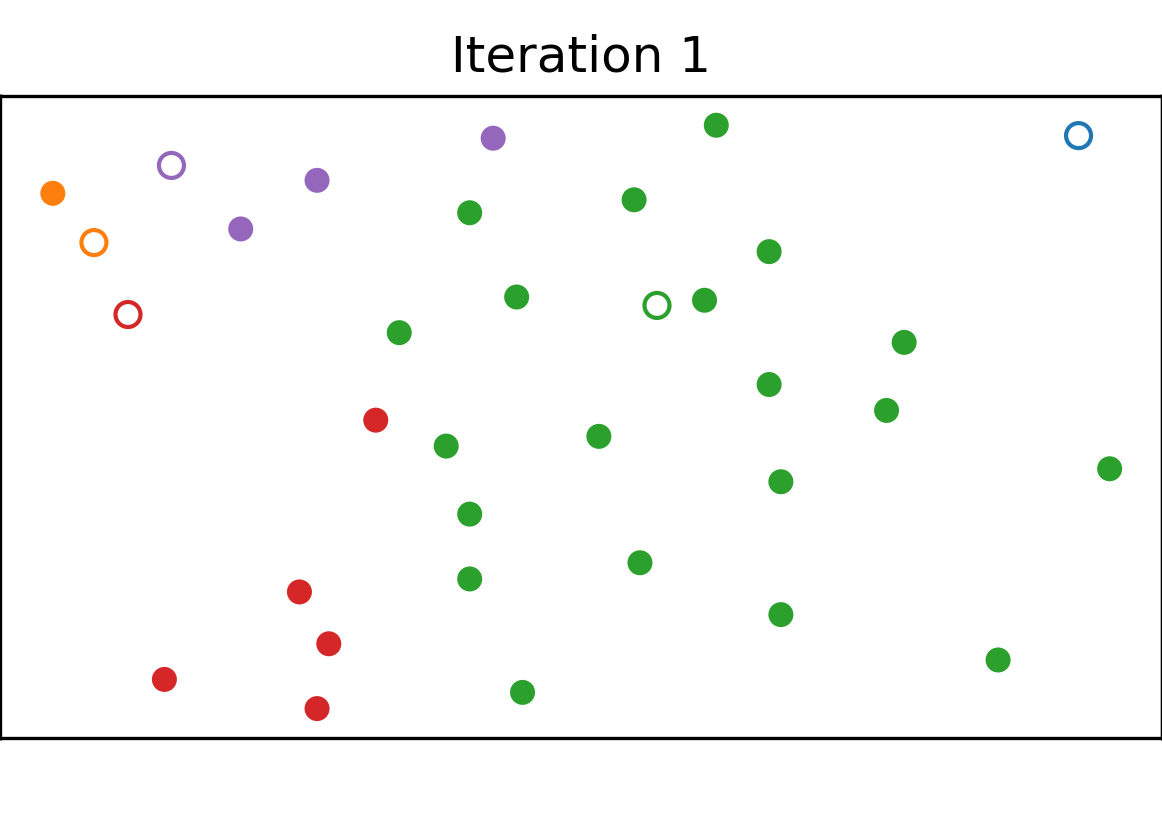
\includegraphics[width=.5\textwidth]{1/1.png}
\end{center}

در تصویر بالا، دایره‌های توپر نماینده شهر‌ها و دایره‌های توخالی نماینده مرکز خوشه‌ها می‌باشند که بر اساس بردار وزن هر خروجی به دست می‌آیند. همه تکرارها را در زیر می‌بینیم.

\LTR
\begin{center}
    \begin{tabular}{ccc}
        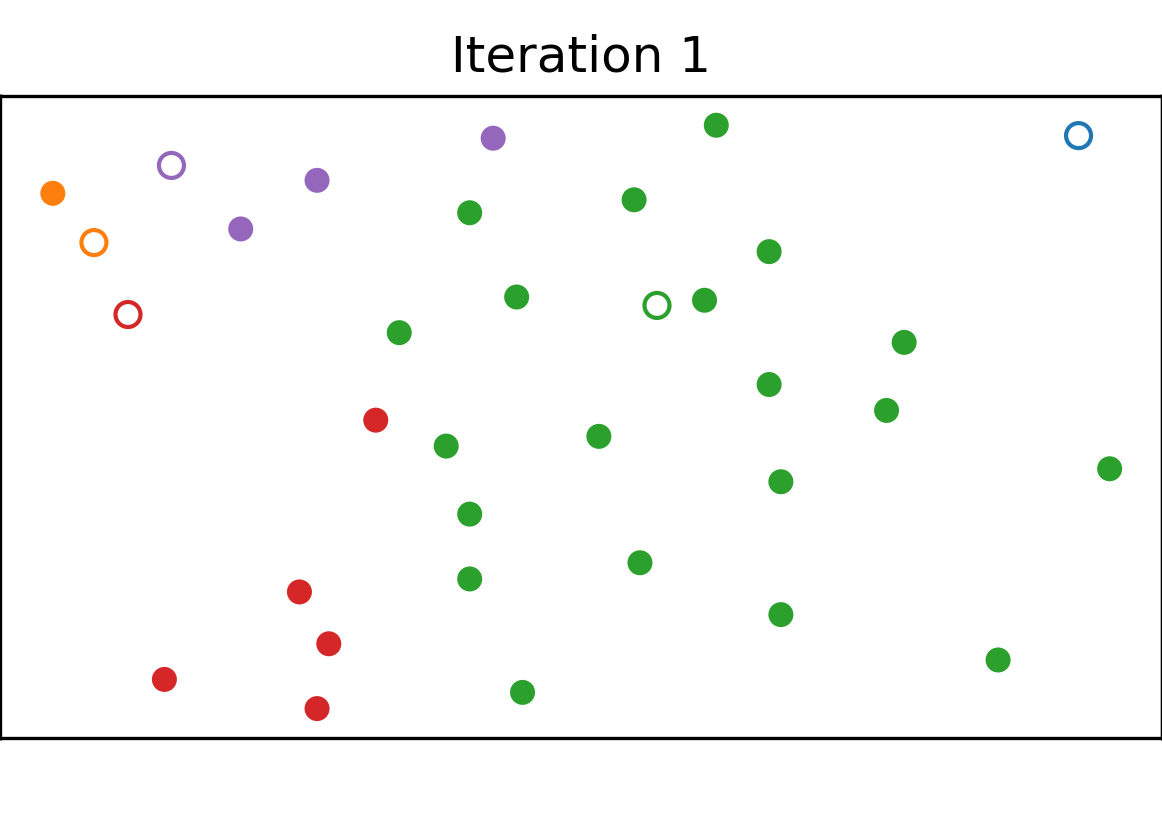
\includegraphics[width=.28\textwidth]{1/1.png} &
        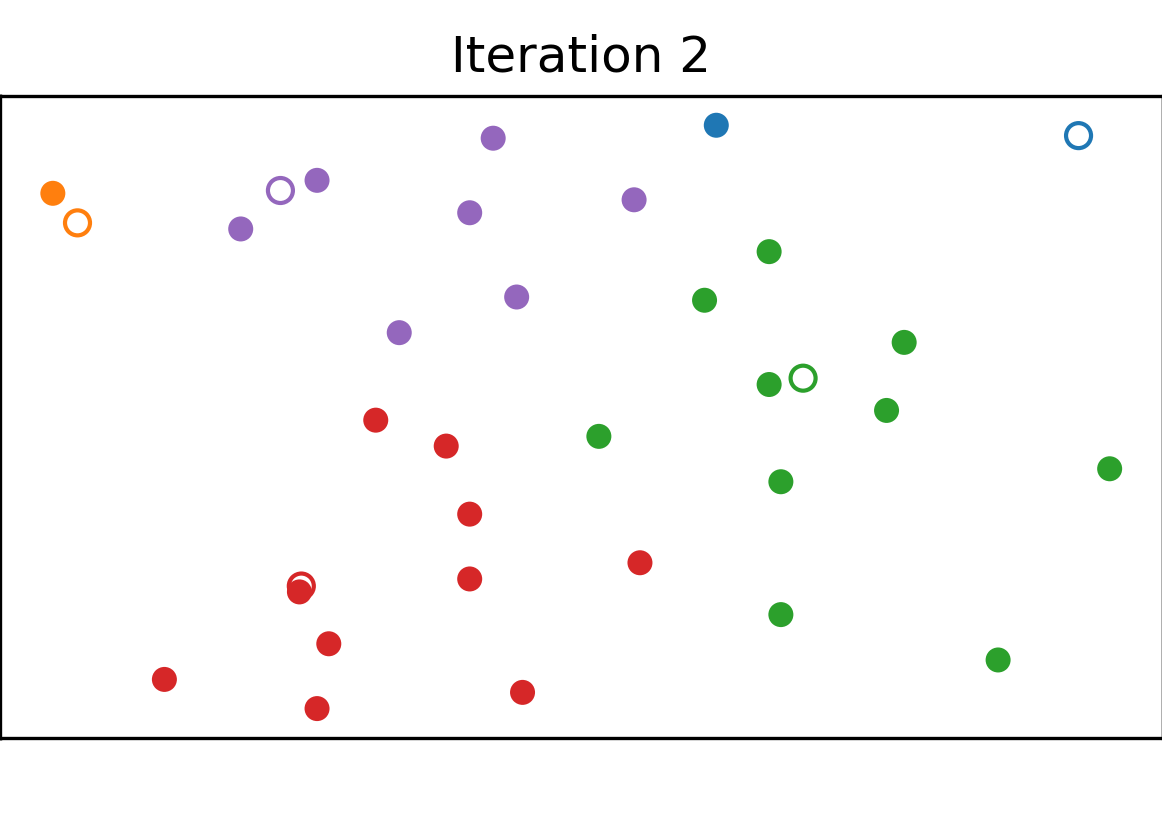
\includegraphics[width=.28\textwidth]{1/2.png} &
        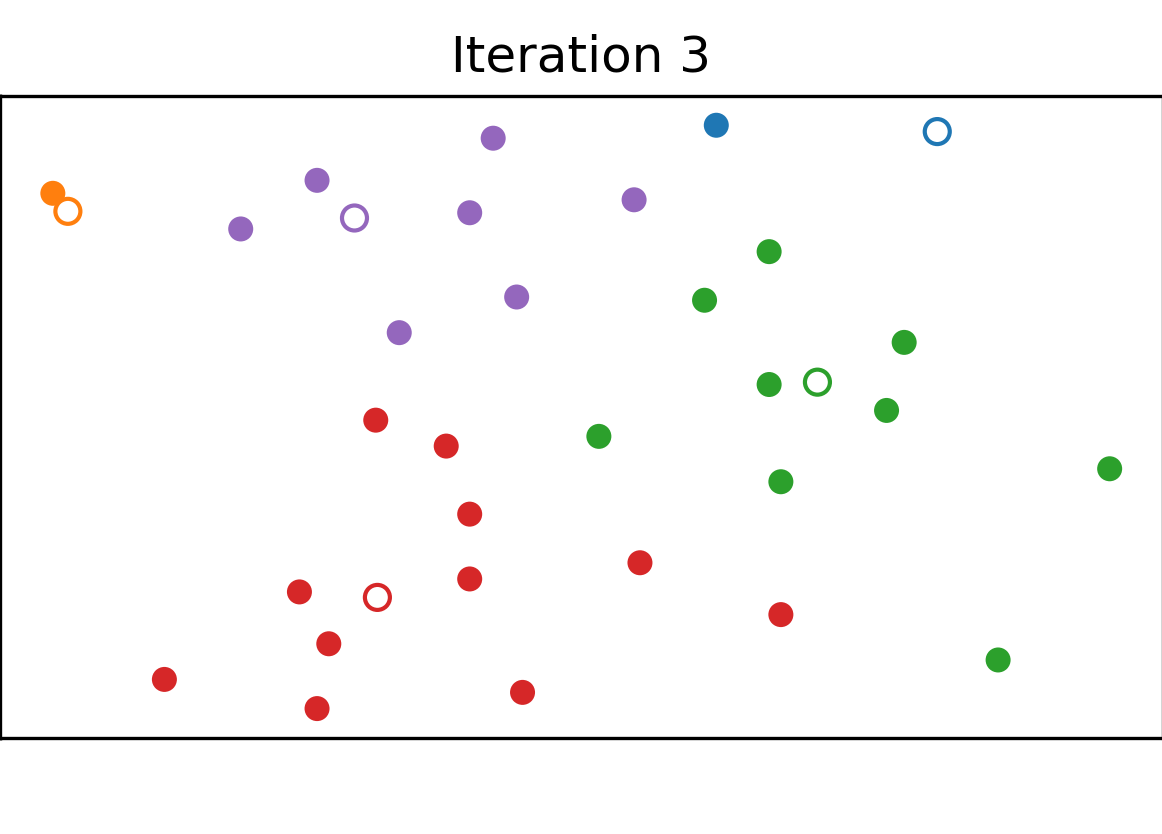
\includegraphics[width=.28\textwidth]{1/3.png}   \\
        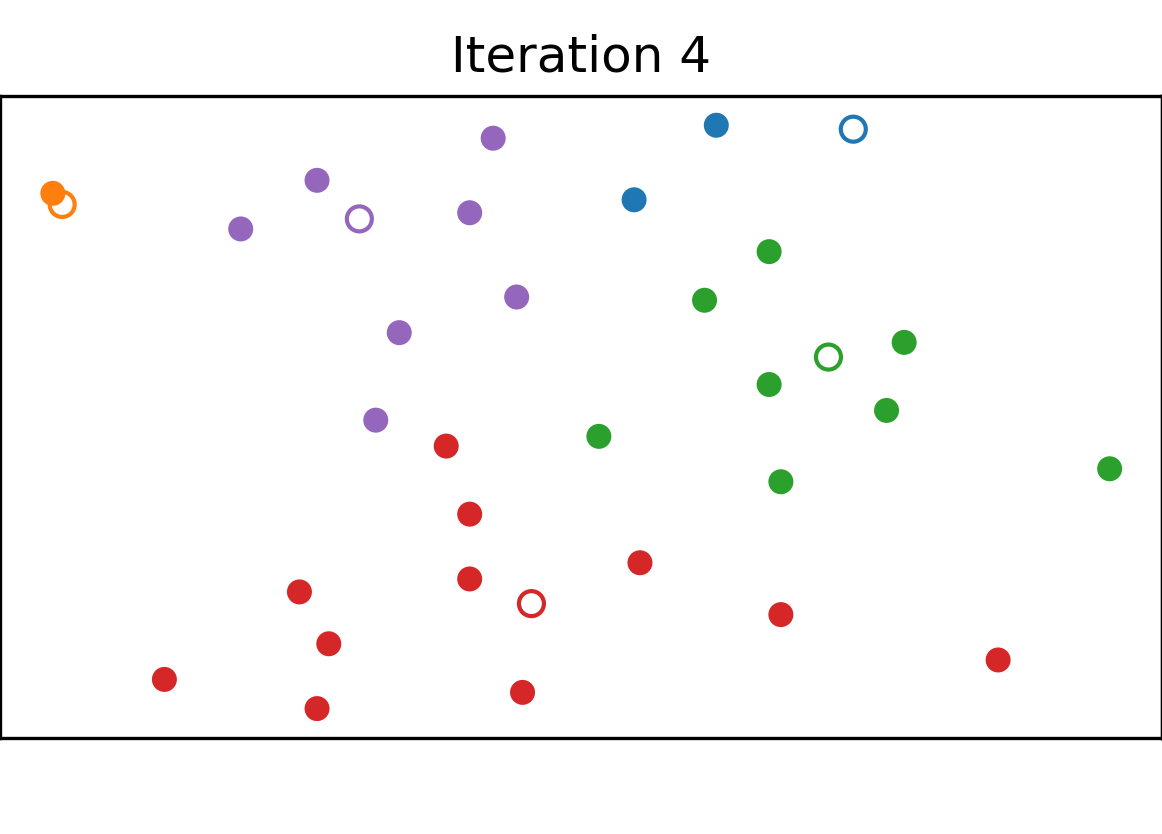
\includegraphics[width=.28\textwidth]{1/4.png} &
        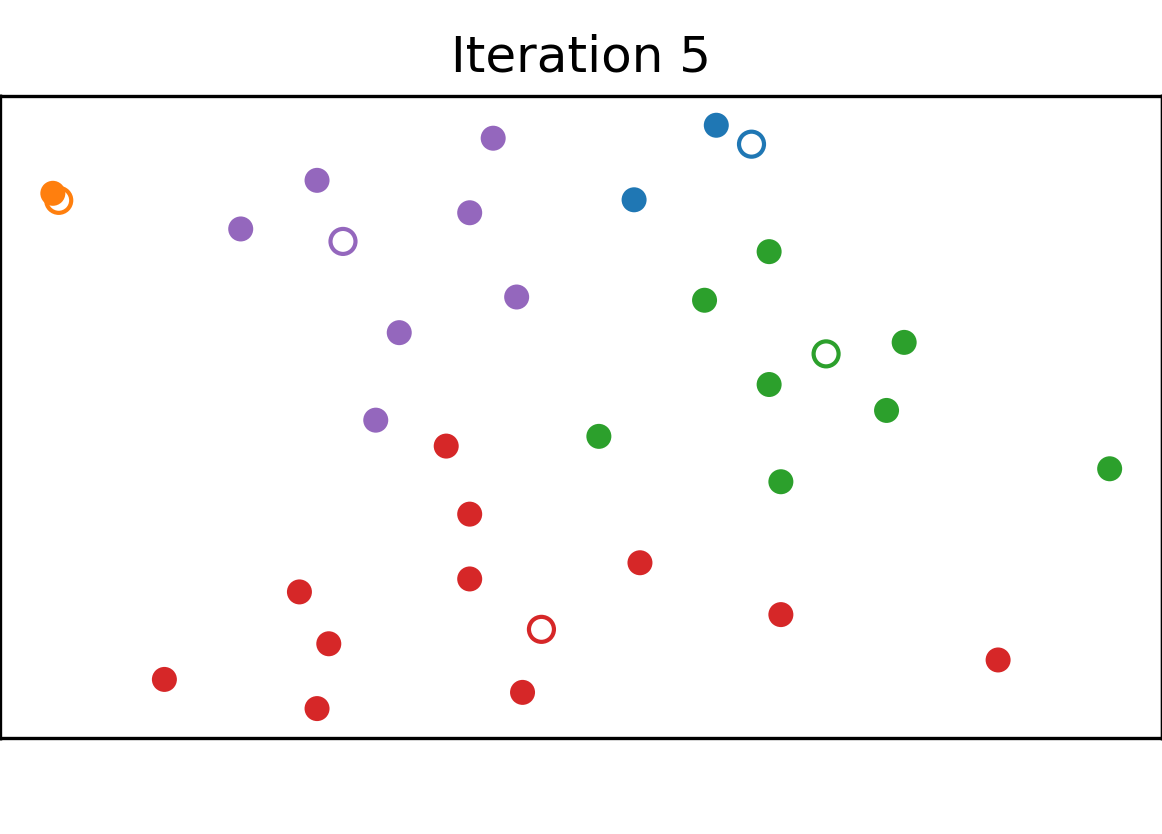
\includegraphics[width=.28\textwidth]{1/5.png} &
        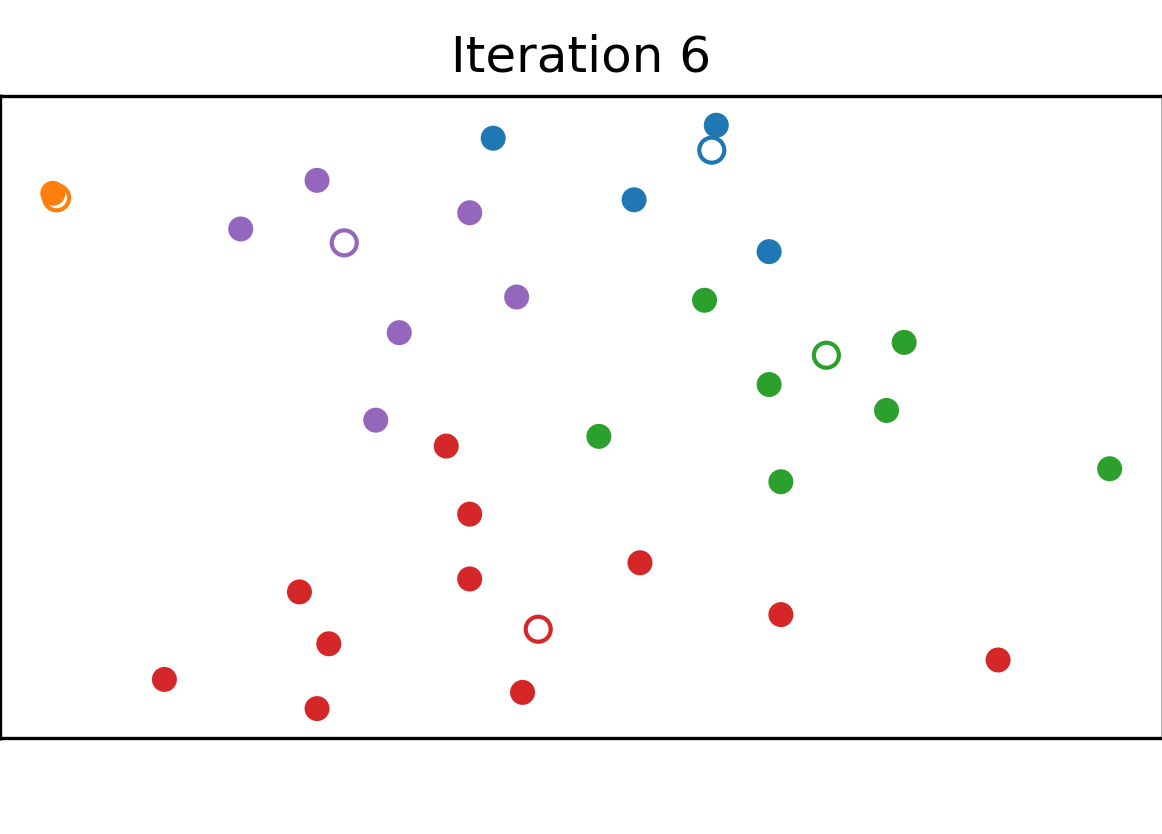
\includegraphics[width=.28\textwidth]{1/6.png}   \\
        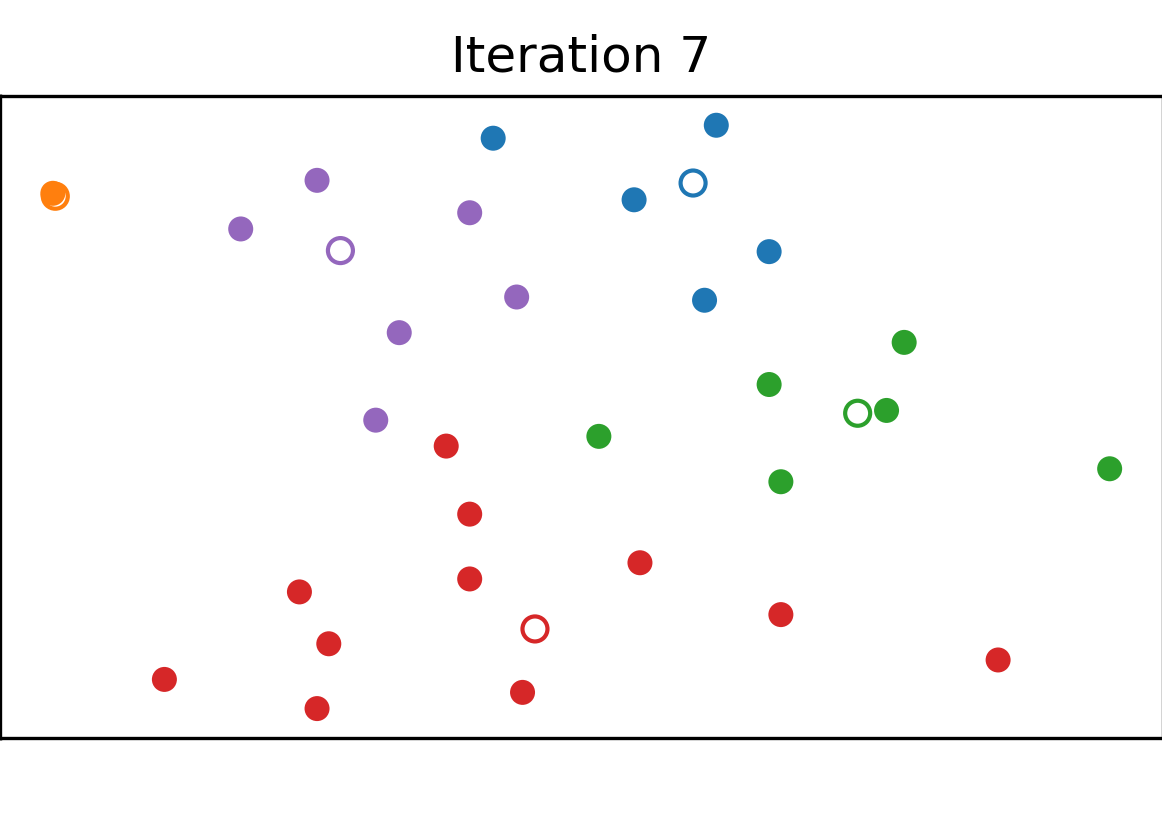
\includegraphics[width=.28\textwidth]{1/7.png} &
        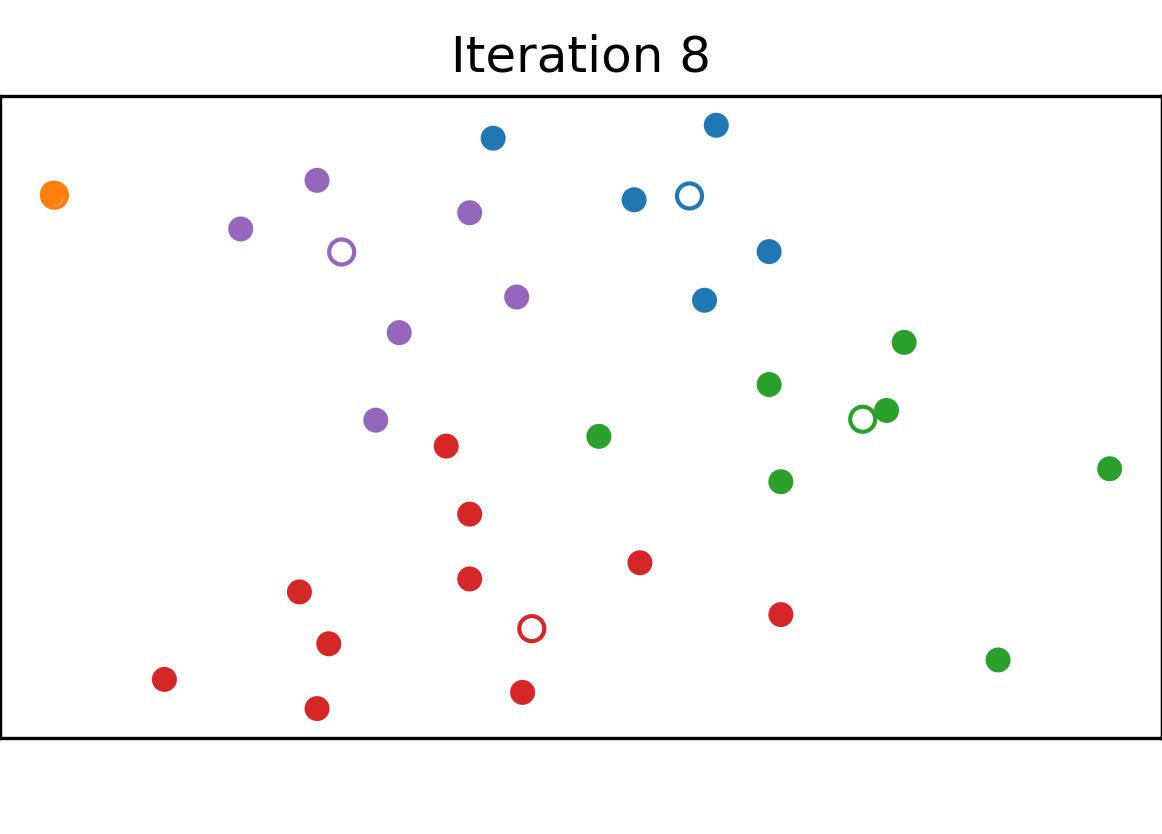
\includegraphics[width=.28\textwidth]{1/8.png} &
        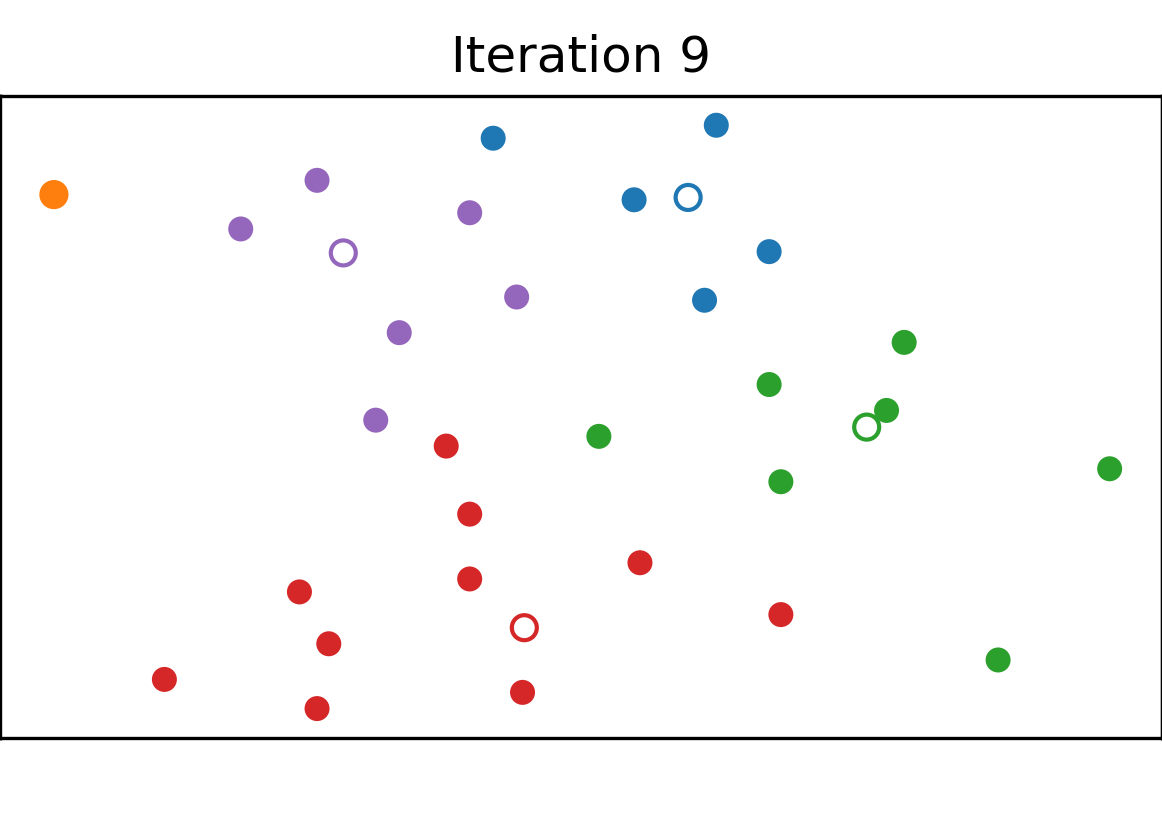
\includegraphics[width=.28\textwidth]{1/9.png}   \\
    \end{tabular}
\end{center}
\RTL

در این مراحل، جابه‌جایی مراکز خوشه‌ها برای رسیدن به حالت بهتر قابل مشاهده می‌باشد.

\section{مسیریابی درون‌خوشه‌ای}

حال که شهرها را خوشه‌بندی کردیم. می‌توانیم یک مسیر خوب درون هر خوشه پیدا کنیم و سپس خوشه‌ها را به یکدیگر متصل کنیم تا پاسخ خوبی برای مسئله فروشنده دوره‌گرد به دست آید. برای این منظور لازم است تا به لیست شهرهای هر خوشه دسترسی داشته باشیم پس ابتدا این لیست را برای هر خوشه تعریف می‌کنیم. (در این قسمت خوشه‌های خالی را در صورت وجود حذف می‌کنیم.)


\LTR
\begin{lstlisting}[language=Python]
clusters = list(filter(lambda x: x, [
    {'cities': [city for city in cities if city['cluster'] == i]}
    for i in range(CLUSTERS_COUNT)
]))
\end{lstlisting}
\RTL

سپس در یک حلقه برای هر یک از خوشه‌ها مراحل زیر را انجام می‌دهیم.

\begin{itemize}
    \item اگر تعداد شهرهای خوشه کمتر از ۷ بود، تمام حالت‌های ممکن مسیر حداکثر $6! = 720$ می‌باشد. تمام این حالات را بررسی می‌کنیم و بهترین مسیر را انتخاب می‌کنیم.
    \item در غیر این صورت، یکی از مسیرها را به صورت تصادفی در نظر می‌گیریم. (این بخش را می‌توان با الگوریتم‌های بهینه‌سازی دیگر ترکیب کرد تا پاسخ بهتری به دست آید.)
    \item مسیر به‌دست‌آمده و هزینه آن برای این خوشه را ذخیره می‌کنیم. همچنین دو سر انتهایی این مسیر را ذخیره می‌کنیم تا بعدا هنگامی که می‌خواهیم دو خوشه را به یکدیگر متصل کنیم از آن استفاده کنیم.
\end{itemize}

پیاده‌سازی این مراحل به صورت زیر خواهد شد.

\LTR
\begin{lstlisting}[language=Python]
for cluster in clusters:
    # If the cluster is small and it is possible, use brute-force and check all permutations and find the best.
    if len(cluster) < 7:
        permutations = list(map(list, itertools.permutations(cluster['cities'])))
        costs = [
            sum([euclidean_distance(p[j]['position'], p[j + 1]['position']) for j in range(len(p) - 1)])
            for p in permutations
        ]
        best_cost = min(costs)
        best_permutation = permutations[costs.index(best_cost)]
    # Else, just use a random permutation. (This part can be better if we use other optimization algorithms as a mix.)
    else:
        best_permutation = cluster['cities'].copy()
        shuffle(best_permutation)
        best_cost = sum([
            euclidean_distance(best_permutation[j]['position'], best_permutation[j + 1]['position'])
            for j in range(len(best_permutation) - 1)
        ])

    # Add this path to roads array
    roads += [(best_permutation[j], best_permutation[j + 1]) for j in range(len(best_permutation) - 1)]

    # Add two endpoints of the path to cluster data for connecting clusters
    cluster['ends'] = (best_permutation[0], best_permutation[-1])

    # Add the cost of this part
    cost += best_cost
\end{lstlisting}
\RTL

نتیجه را ترسیم می‌کنیم

\LTR
\begin{lstlisting}[language=Python]
visualizer.add(cities, roads=roads, title=f'Intracluster Roads')
\end{lstlisting}
\RTL

\begin{center}
    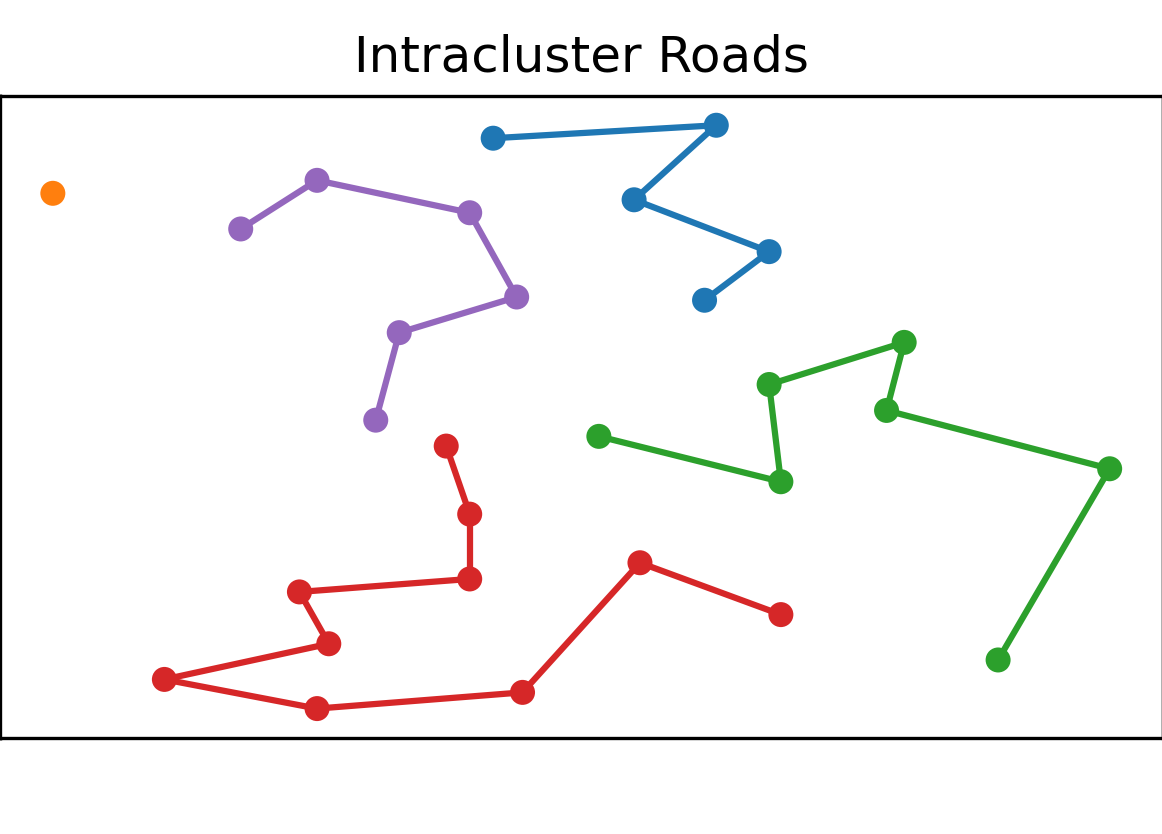
\includegraphics[width=.5\textwidth]{1/10.png}
\end{center}

\section{مسیریابی بین‌خوشه‌ای}

برای مسیریابی بین خوشه‌ای از آنجا که تنها ۵ خوشه داریم می‌توانیم تمام حالات را بررسی کنیم. برای ایجاد تمام حالات باید تمام جایگشت‌های خوشه‌ها را در نظر بگیریم اما چون روی یک دور قرار می‌گیرند جایگشت‌های دوری را یکی در نظر بگیریم همچنین جایشگتی مانند
$1, 2, 3, 4, 5$
و
$5, 4, 3, 2, 1$
نیز یکسان می‌باشند که آینه یکدیگر می‌باشند پس در کل
$\frac{5!}{5 \times 2} = 12$
جایگشت مختلف داریم. که به کمک توابع زیر این جایگشت‌ها را می‌سازیم.

\LTR
\begin{lstlisting}[language=Python]
def cmp(n):
    ''' Circular Mirrorable Permutations of numbers 1 to n '''
    if n == 3:
        return [[1, 2, 3]]

    ps = cmp(n - 1)
    r = []
    for p in ps:
        for i in range(n - 1):
            t = p.copy()
            t.insert(i, n)
            r.append(t)
    return r


def cm_permutations(l):
    n = len(l)
    return [[l[p[i] - 1] for i in range(n)] for p in cmp(n)]
\end{lstlisting}
\RTL

اما یک نکته دیگر که باید به آن توجه کنیم این است که هر خوشه دو سر دارد که باید تصمیم بگیریم از کدام سر به خوشه بعدی متصل شود. اگر یک سر را صفر و سر دیگر را یک بنامیم برای هر خوشه دو حالت داریم که کدام سر آن به خوشه بعدی متصل می‌شود. اما سری که به خوشه قبلی متصل می‌شود به طور منحصربه‌فردی تعیین می‌شود. (همان سری که به بعدی وصل نمی‌شود) پس به تعداد کدهای باینری به طول تعداد کلاسترها حالت مختلف برای وصل کردن داریم که برابر است با
$2^5$
و لذا کل حالات برابر
$2^5 \times 12 = 384$
می‌باشد. برای ایجاد همه این حالات از کد زیر استفاده می‌کنیم.

\LTR
\begin{lstlisting}[language=Python]
options = [list(map(int, format(i, f'0{CLUSTERS_COUNT}b'))) for i in range(2 ** CLUSTERS_COUNT)]
\end{lstlisting}
\RTL

حال می‌توانیم همه حالات را بررسی کنیم و بهترین حالت را انتخاب کنیم.

\LTR
\begin{lstlisting}[language=Python]
for p in permutations:
for option in options:
    po_cost = 0
    po_roads = []
    for j in range(len(p)):
        po_cost += euclidean_distance(p[j]['ends'][1 - option[j]]['position'],
                                        p[j - 1]['ends'][option[j - 1]]['position'])
        po_roads += [(p[j]['ends'][1 - option[j]], p[j - 1]['ends'][option[j - 1]])]
    if intercluster_cost is None or po_cost < intercluster_cost:
        intercluster_cost = po_cost
        intercluster_roads = po_roads
\end{lstlisting}
\RTL

نهایتا جاده‌های بین‌خوشه‌ای را به لیست کل جاده‌ها اضافه می‌کنیم و هزینه آن را به کل هزینه‌ها و سپس نقشه جدید به همراه جاده‌های بین‌خوشه‌ای را رسم می‌کنیم.

\LTR
\begin{lstlisting}[language=Python]
roads += intercluster_roads
cost += intercluster_cost

visualizer.add(cities, roads=roads, title=f'All Roads')
\end{lstlisting}
\RTL

که تصویر آن به صورت زیر خواهد شد.

\begin{center}
    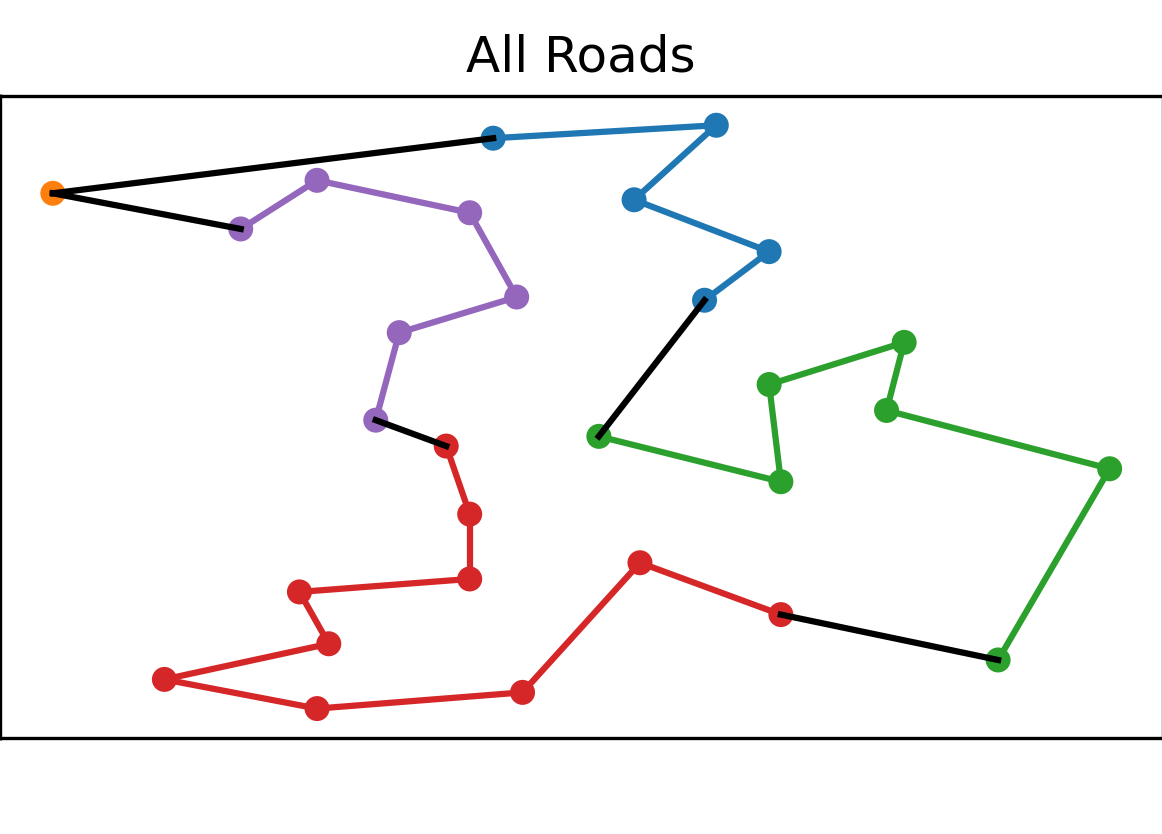
\includegraphics[width=.5\textwidth]{1/11.png}
\end{center}

\section{پاسخ نهایی}

در نهایت هزینه کل را چاپ می‌کنیم و تمام تصاویر را در کنار هم قرار می‌دهیم.

\LTR
\begin{lstlisting}[language=Python]
visualizer.fig.suptitle(f'Cost = {cost}')

visualizer.show()    
\end{lstlisting}
\RTL


\begin{center}
    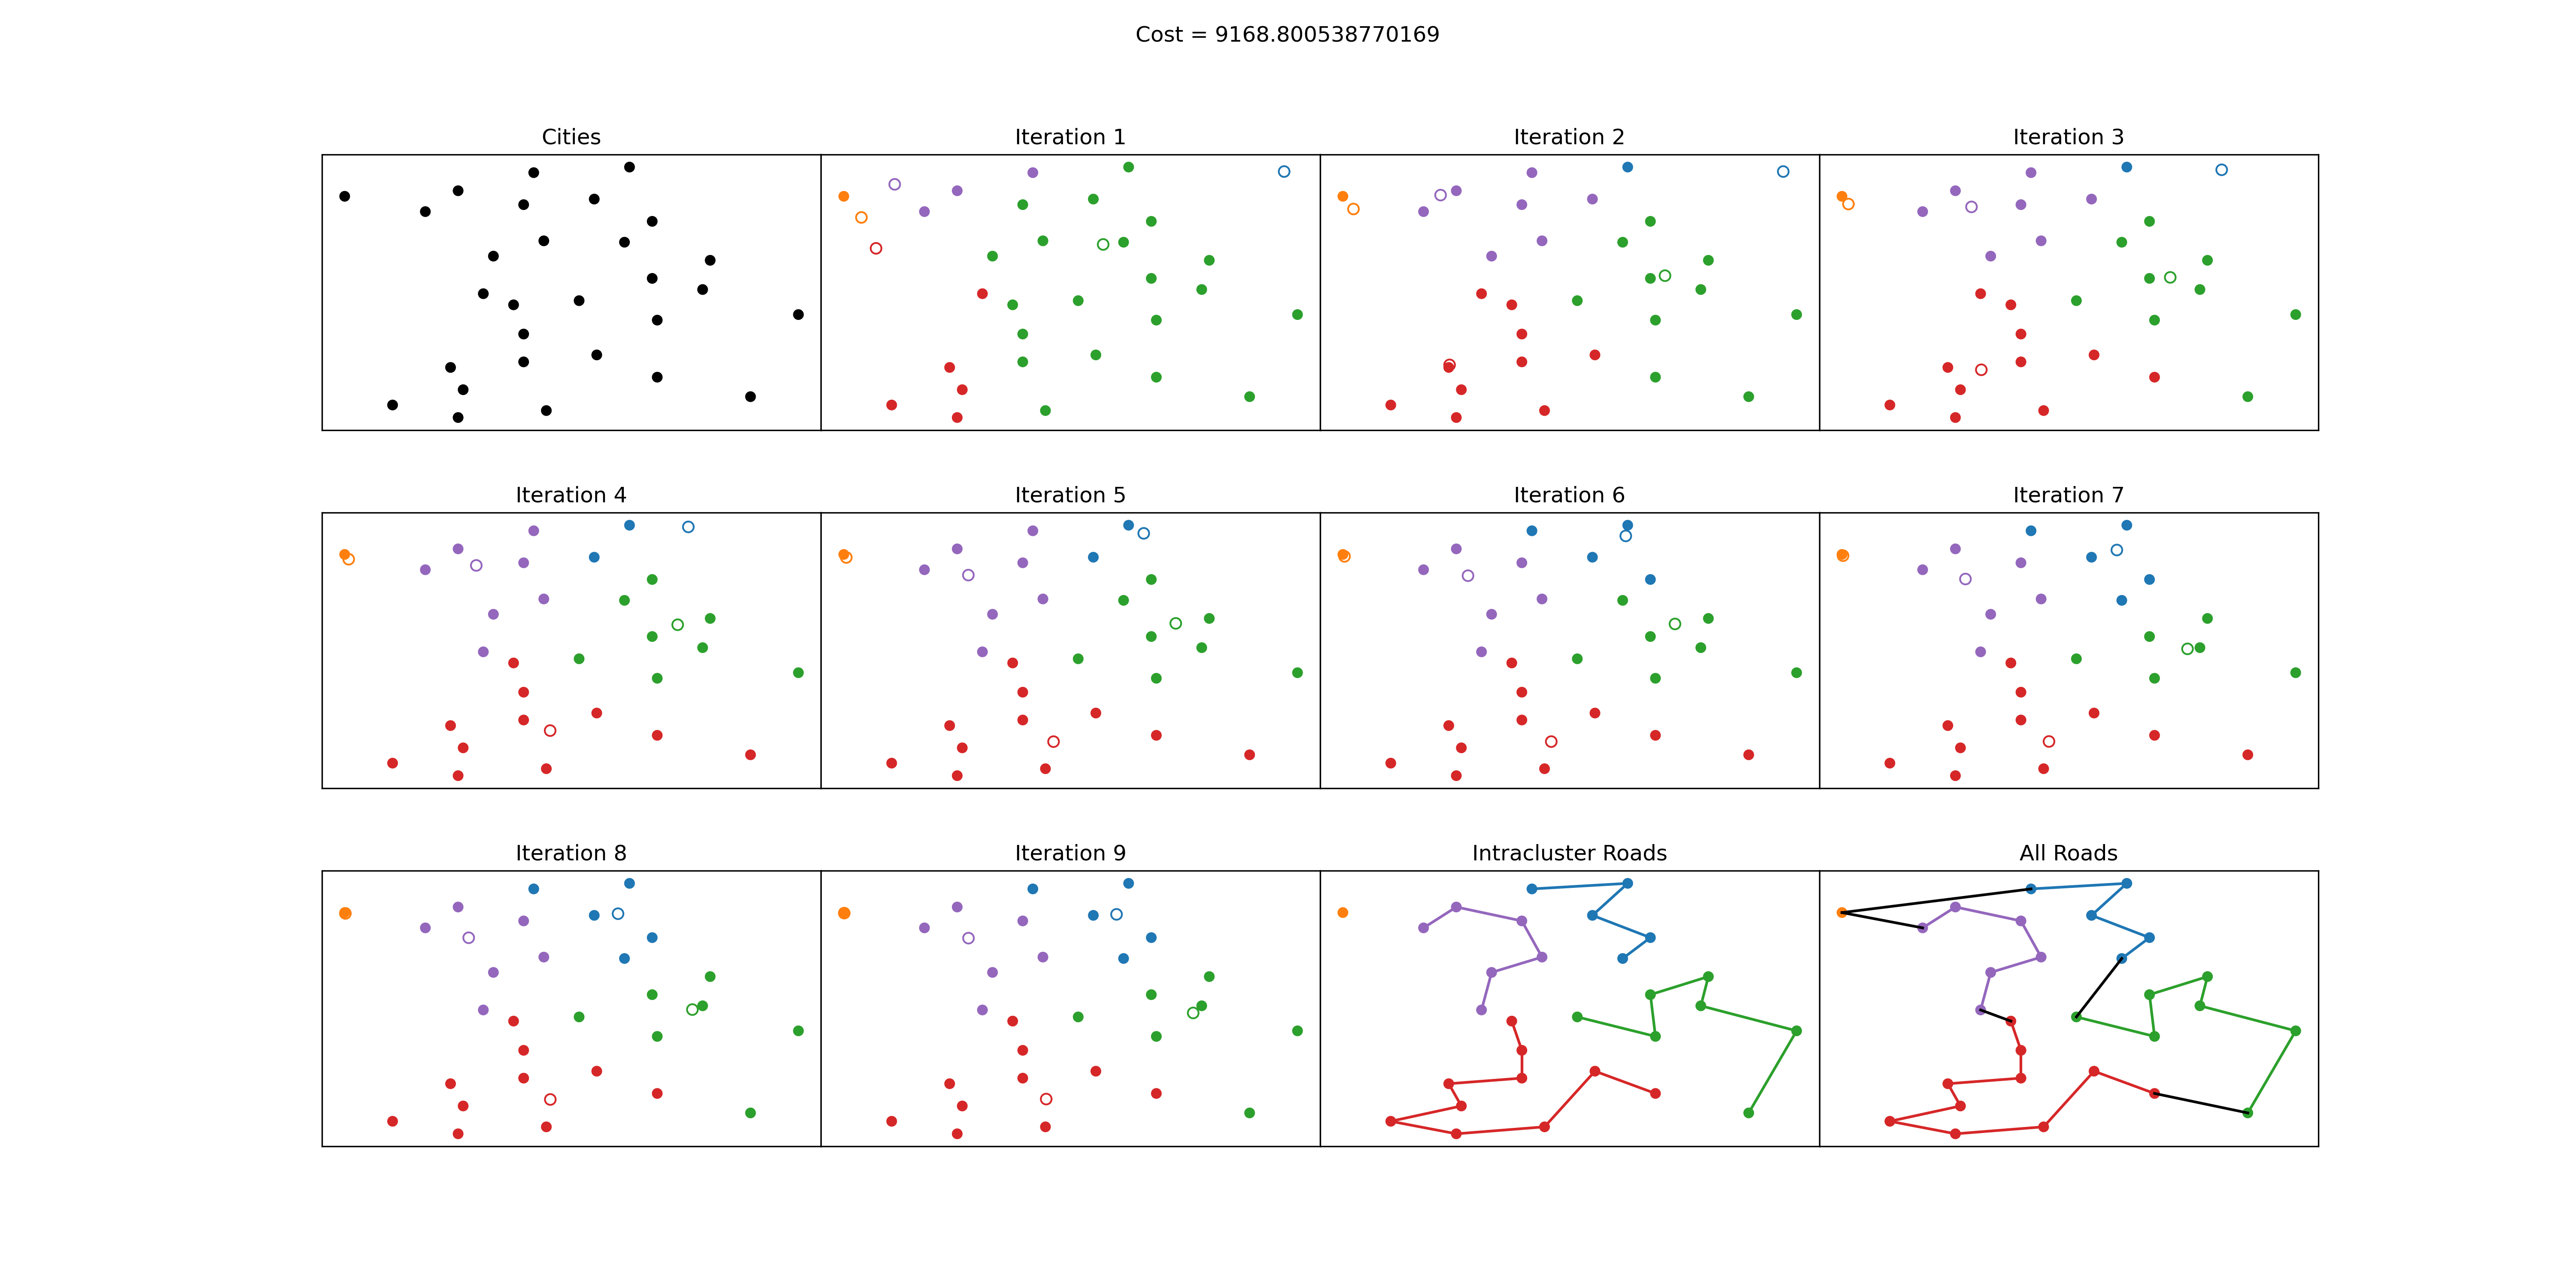
\includegraphics[width=\textwidth]{1/all.png}
\end{center}

همانطور که می‌بینیم هزینه کل
$9168$
به دست آمده و می‌دانیم بهترین پاسخ به این مسئله
$9074$
می‌باشد پس پاسخ قابل قبولی به دست آوردیم.

\end{document}